\section{Ações de controle}


\begin{frame}{Ações de controle}
	\begin{block}{Introdução}
		\begin{itemize}
			\item Não é desejável que o controle de uma variável seja \textbf{errôneo} ou que \textbf{desgaste} os componentes físicos usados no processo.
			\item As \textbf{ações de controle} são referentes a \textbf{maneira} que vamos variar nossa \textbf{variável manipulada}, podendo usar um simples método \textbf{ON-OFF}, ou algo mais \textbf{sofisticado}, a fim de \textbf{otimizar} o controle.
			\item O controle é feito através dos \textbf{Elementos Finais de Controle} (EFCs), chamados \textbf{atuadores} nos diagramas de blocos.
			\item Os EFCs são equipamentos \textbf{complexos}, e que devem ser estudados a parte, mas no estudo do controle é importante saber algumas características sobre eles:
			\begin{itemize}
				\item Os EFCs podem atuar na variável manipulada de \textbf{diversas formas} (controlando vazão, temperatura...).
				\item Os EFCs possuem \textbf{faixas de atuação} (uma válvula pode abrir-se entre 0\% e 100\%).
			\end{itemize}
		\end{itemize}
	\end{block}
\end{frame}


\begin{frame}{Liga-desliga (ON-OFF)}
	\begin{block}{Introdução - Exemplo \#01}
		O controle ON-OFF é \textbf{o mais simples} possível, trata-se simplesmente de controlar um equipamento ligando-o e desligando-o \textbf{conforme o necessário}.
		
		\smallskip
		
		Para visualizar isso melhor, imagine:
		\begin{itemize}
			\item Você deseja que a temperatura de um cômodo \textbf{permaneça} em \textbf{\SI{22}{\degreeCelsius}}.
			\item Para isso, o controlador de um ar condicionado tem as seguintes instruções:
			\begin{enumerate}
				\item \normalsize Caso esteja \textbf{desligado}:
				\begin{itemize}
					\item \small Se a temperatura do cômodo estiver \textbf{acima} de \SI{22}{\degreeCelsius}, \textbf{ligue o compressor}.
					\item \small Se a temperatura do cômodo estiver \textbf{igual ou abaixo} de \SI{22}{\degreeCelsius}, \textbf{não faça nada}.
				\end{itemize}
				\item \normalsize Caso esteja \textbf{ligado}:
				\begin{itemize}
					\item \small Se a temperatura do cômodo estiver \textbf{acima} de \SI{22}{\degreeCelsius}, \textbf{não faça nada}.
					\item \small Se a temperatura do cômodo estiver \textbf{igual ou abaixo} de \SI{22}{\degreeCelsius}, \textbf{desligue o compressor}.
				\end{itemize}
			\end{enumerate}
			
		\end{itemize}
	\end{block}
\end{frame}

% sensor -> termostato
% comparação
% controlador -> chave seletora
% atuador -> compressor
% planta -> refrigerador

\begin{frame}{Liga-desliga (ON-OFF)}
	\begin{block}{Problema - Exemplo \#01}
		No caso do nosso ar condicionado, estas condições podem ser acomodadas por um \textbf{termostato}, mas temos alguns \textbf{problemas} de início:
		\begin{itemize}
			\item Caso o termostato meça \textbf{\SI{22.1}{\degreeCelsius}} e o compressor estiver desligado, vai \textbf{ligar}.
			\item Quando a temperatura diminuir para \textbf{\SI{21.9}{\degreeCelsius}}, pela lógica que utilizamos, o compressor deve \textbf{desligar} novamente.
			\item E esse processo se repete \textbf{infinitamente}, sendo cada vez \textbf{mais frequente} dependendo da \textbf{precisão} do termostato (liga em \SI{22.0001}{\degreeCelsius} e desliga em \SI{21.9999}{\degreeCelsius}).
		\end{itemize}
		Se nosso controle ON-OFF for feito dessa maneira, nosso compressor estará \textbf{quebrado} em menos de algumas horas.
	\end{block}
\end{frame}


\begin{frame}{Liga-desliga (ON-OFF)}
	\begin{block}{Histerese - Exemplo \#01}
		\begin{itemize}
			\item Para lidar com esse problema, devido ao \textbf{ruído} presente na região onde o \textbf{erro} está \textbf{perto de zero}, podemos utilizar a \textbf{histerese}.
			\item Efetivamente, a histerese num sistema \textbf{muda seu comportamento} quando o valor de entrada está \textbf{subindo} e quando está \textbf{descendo}.
			\item No caso do ar condicionado:
			\begin{enumerate}
				\item \normalsize Aumenta sua tolerância quando a temperatura aumenta (só vai ligar quando chegar aos \SI{23}{\degreeCelsius}).
				\item \normalsize Aumenta sua resistência para desligar (só vai desligar quando estiver medindo \SI{21}{\degreeCelsius}).
			\end{enumerate}
		\end{itemize}
		
	\end{block}
	
\end{frame}


\begin{frame}{Liga-desliga (ON-OFF)}
	\centering
	\includegraphics[width=0.7\linewidth]{Figuras/Ch12/fig1}
	
	Gráfico com histerese
\end{frame}


\begin{frame}{Liga-desliga (ON-OFF)}
	\centering
	\includegraphics[width=0.65\linewidth]{Figuras/Ch12/fig2}
	
	Gráfico de um controlador ON-OFF
\end{frame}


\begin{frame}{Ação proporcional (P)}
	\begin{block}{Introdução}
		\begin{itemize}
			\item É considerada a \textbf{evolução} do controle liga-desliga.
			\item Esse tipo de controle atua \textbf{de acordo} com o erro, \textbf{proporcionalmente} a ele.
			\item Utilizando o controle proporcional, é possível evitar os \textbf{movimentos bruscos} provocados pela ação ON-OFF, de forma a \textbf{aumentar} a vida-útil dos equipamentos utilizados.
			\item A ideia básica é \textbf{multiplicar} o erro por um valor fixo, \textbf{proporcional à velocidade que desejamos que o erro se corrija}, mas que ao mesmo tempo poderá fazer com que a variável controlada \textbf{ultrapasse} o \textit{setpoint}.
		\end{itemize}
	\end{block}
\end{frame}


\begin{frame}{Ação proporcional (P)}
	\begin{block}{Exemplo \#01}
		\begin{itemize}
			\item Imagine um forno industrial que deve se manter à \SI{200}{\degreeCelsius}.
			\item Dependendo da hora do dia, a carga desse forno \textbf{varia} radicalmente, sendo necessárias correções \textbf{precisas} e \textbf{rápidas}, mas que também \textbf{preservem o equipamento}, que funciona sem parar.
		\end{itemize}
	\end{block}

	\centering
	\includegraphics[height=0.55\textheight]{Figuras/Ch12/fig4}
\end{frame}


\begin{frame}{Ação proporcional (P)}
	\begin{block}{Exemplo \#01}
		\begin{itemize}
			\item A regularem da temperatura no forno é feita utilizando um \textbf{fole} com um \textbf{fluido} que se expande \textbf{de acordo com a temperatura do forno}.
			\item A haste conectada ao fole é presa à válvula que regula o gás que entra no forno, através de um esquema de \textbf{alavanca}.
			\item A \textbf{posição de apoio} dessa alavanca é equivalente ao \textbf{ganho} do controlador proporcional, que é a própria alavanca.
		\end{itemize}
	\end{block}

	\medskip

	\centering
	\includegraphics[height=0.3\textheight]{Figuras/Ch12/fig4n1}
\end{frame}


\begin{frame}{Ação proporcional (P)}
	\begin{block}{Ganho - Exemplo \#01}
		\begin{itemize}
			\item O ganho representa a \textbf{rapidez de resposta do sistema}: quanto \textbf{maior} o ganho, \textbf{maior} a rapidez com que irá \textbf{responder} ao erro.
		\end{itemize}
	\end{block}

	\bigskip
	
	\centering
	\includegraphics[width=0.9\linewidth]{Figuras/Ch12/fig4n2}
\end{frame}


\begin{frame}{Ação proporcional (P)}
	\begin{block}{Ganho}
		\begin{itemize}
			\item O valor do ganho nos permite controlar qual \textbf{faixa de variação} da variável medida iremos atuar sobre.
			\item A \textbf{banda proporcional}, no controle proporcional, é o nome dado à essa nova faixa, que obedece à relação\[ BP=\dfrac{100\%}{K_p} \]
			\item Uma $ BP $ de 20\% é lida como: a \textbf{variação máxima} necessária para fazer nosso atuador variar de completamente \textbf{aberto} para completamente \textbf{fechado} é de 20\% da faixa \textbf{em relação ao \textit{setpoint}}.
		\end{itemize}
	\end{block}
\end{frame}


\begin{frame}{Ação proporcional (P)}
	\begin{block}{Gráfico $ VC \times VM $}
		\[ BP=100\% \]
	\end{block}

\medskip

\centering

\scalebox{0.8}{
	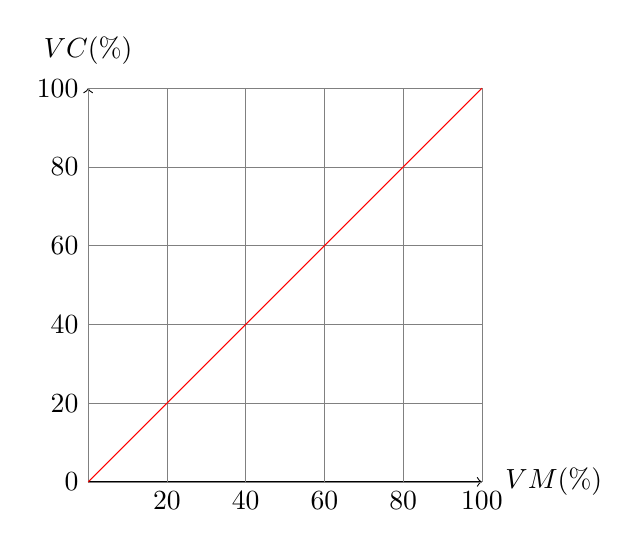
\begin{tikzpicture}[x=0.5cm,y=0.5cm]
		\draw[->] (0,0) -- (0,10) node[above=5pt] {$ VC(\%) $};
		\draw[->] (0,0) -- (10,0) node[right=5pt] {$ VM(\%) $};
		
		\draw (0,0) node[left] {$ 0 $};
		
		\foreach \x in {2,4,...,10}{
			\draw (0,\x) node[left] {$ \x 0 $};
			\draw (\x,0) node[below] {$ \x 0 $};
		}
		
		\draw[help lines, step=1cm] (0,0) grid (10,10);
		
		\draw[red] (0,0) -- (10,10);
	\end{tikzpicture}}
\end{frame}


\begin{frame}{Ação proporcional (P)}
	\begin{block}{Gráfico $ VC \times VM $}
		\[ BP=60\% \]
	\end{block}
	
	\medskip
	
	\centering
	
	\scalebox{0.8}{
		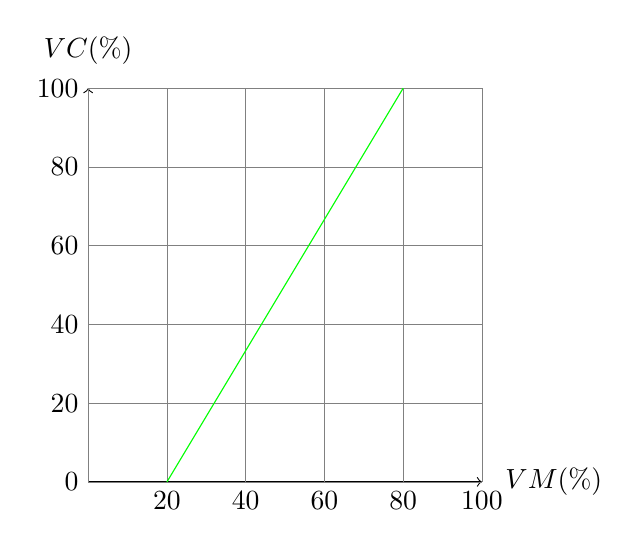
\begin{tikzpicture}[x=0.5cm,y=0.5cm]
		\draw[->] (0,0) -- (0,10) node[above=5pt] {$ VC(\%) $};
		\draw[->] (0,0) -- (10,0) node[right=5pt] {$ VM(\%) $};
		
		\draw (0,0) node[left] {$ 0 $};
		
		\foreach \x in {2,4,...,10}{
			\draw (0,\x) node[left] {$ \x 0 $};
			\draw (\x,0) node[below] {$ \x 0 $};
		}
		
		\draw[help lines, step=1cm] (0,0) grid (10,10);
		
		\draw[green] (2,0) -- (8,10);
		\end{tikzpicture}}
\end{frame}


\begin{frame}{Ação proporcional (P)}
	\begin{block}{Relação proporcional}
		\begin{itemize}
			\item A ação de controle proporcional segue a relação:
			\[ C_p(t) = K_p\cdot E(t) \]
			onde $ C_p $ é a saída da componente proporcional no tempo, $ K_p $ é o ganho, e $ E(t) $ é o erro no tempo, calculado por
			\[ E(t)=SP-VC(t) \]
			sendo $ SP $ o \textit{setpoint} e $ VC $ o valor medido da variável controlada.
		\end{itemize}
	\end{block}
\end{frame}


\begin{frame}{Ação proporcional (P)}
	\begin{block}{Introdução - Ação direta x ação reversa}
		Após a \textbf{estabilização} no \textit{setpoint}, havendo \textbf{distúrbios} no processo, podemos identificar o \textit{off-set}, que é o \textbf{erro remanescente} deixado pela ação proporcional:
		\begin{enumerate}
			\item Caso $ E(t)<0 $ - \textit{off-set} positivo: passamos do \textit{setpoint}.
			\item Caso $ E(t)>0 $ - \textit{off-set} negativo: estamos abaixo do \textit{setpoint}.
		\end{enumerate}
		\begin{itemize}
			\item À medida que \textbf{aumentamos} o ganho proporcional, \textbf{menor} é o erro de offset, porém um ganho \textbf{muito	alto} aproxima o sistema de um \textbf{controle ON-OFF}.
			\item Sistemas com tempo morto apresentam \textbf{maior} erro de \textit{off-set}.
		\end{itemize}
	\end{block}
\end{frame}


\begin{frame}{Ação proporcional (P)}
	\begin{block}{Ação direta x ação reversa}
		\begin{itemize}
			\item No entanto, isso não nos informa em \textit{como} controlar o atuador, que pode ser \textbf{inversamente proporcional} à VC.
			\item E então, temos os conceitos de \textbf{ação direta} e \textbf{ação reversa}, que se referem ao \textbf{sinal} do ganho utilizado em nosso controlador.
		\end{itemize}
	\end{block}

	\medskip
	
	\resizebox{\textwidth}{!}{
	\begin{tabular}{llc}
			\toprule
			\thead{\normalsize Ação} & \thead{\normalsize Situação} & \thead{\normalsize Saída do controlador}\\ \midrule
			\multirow{2}{*}{Direta} & $ E(t)\bm{<}0 $ - \textit{Off-set} \textbf{positivo} & $ VM\bm{>}0 $\\
									& $ E(t)\bm{>}0 $ - \textit{Off-set} \textbf{negativo} & $ VM\bm{<}0 $\\ \midrule
			\multirow{2}{*}{Reversa}& $ E(t)\bm{<}0 $ - \textit{Off-set} \textbf{positivo} & $ VM\bm{<}0 $\\
									& $ E(t)\bm{>}0 $ - \textit{Off-set} \textbf{negativo} & $ VM\bm{>}0 $\\ \bottomrule
	\end{tabular}}
\end{frame}


\begin{frame}{Ação integral (I)}
	\begin{block}{Introdução}
		\begin{itemize}
			\item Como um primeiro passo na correção do \textit{off-set}, podemos usar a \textbf{ação integral}.
			\item Uma forma de alterar o \textit{off-set} sem mudar o ganho proporcional é \textbf{mudar o \textit{setpoint}} para compensar o erro, mas isso é \textbf{inexato} e pode ser \textbf{demorado}.
			\item A ação de controle integral realiza um ajuste \textbf{automático}, corrigindo a saída do controlador conforme o erro não for corrigido \textbf{durante a passagem do tempo}.
			\item Isso significa que, se o controlador proporcional \textbf{parar de corrigir} num determinado momento, com o erro de \textit{off-set} presente, o controlador integral vai atuar sob esse valor até \textbf{eliminá-lo}.
			\item A ação integral \textbf{não é, isoladamente, uma técnica de controle}, pois não pode ser empregada estando separada de uma ação proporcional.
		\end{itemize}
	\end{block}
\end{frame}


\begin{frame}{Controlador proporcional integral (PI)}
	\begin{block}{Introdução}
		\begin{itemize}
			\item Esse controlador irá atuar proporcionalmente em grande parte do tempo, corrigindo o erro \textbf{rápida} e \textbf{efetivamente}.
			\item Porém, ao deixar um \textit{off-set} em relação ao \textit{setpoint}, a ação integral irá atuar de forma \textbf{gradual}, e corrigirá, também, esse erro, que não pode ser corrigido de forma ideal pela ação proporcional.
		\end{itemize}
	\end{block}
\end{frame}


\begin{frame}{Controlador proporcional integral (PI)}
	\begin{block}{Exemplo \#01}
		Para ilustrar melhor a diferença e a utilidade de um controlador PI quando comparado à um controlador P, imagine a seguinte situação:
		\begin{itemize}
			\item Você quer que seu drone fique \textbf{suspenso} à uma altura de \textbf{\SI{15}{\meter}} sobre o solo e, para isso, usa um controlador \textbf{proporcional}.
			\item Os \SI{15}{\meter} são nosso \textbf{\textit{setpoint}} e a \textbf{velocidade das hélices} do drone é nossa \textbf{variável manipulada}.
		\end{itemize}
	\end{block}

	\centering
	\includegraphics[width=0.4\linewidth]{Figuras/Ch12/fig4n3}
\end{frame}


\begin{frame}{Controlador proporcional integral (PI)}
	\begin{block}{Exemplo \#01}
		\begin{itemize}
			\item No começo, o erro é \textbf{grande} e, portanto, a saída para as hélices é \textbf{grande}, fazendo o drone se levantar \textbf{rapidamente}.
			\item Depois, conforme se eleva no ar, com a \textbf{diminuição do erro}, o sinal de saída deve sofrer uma queda \textbf{abrupta}, tendendo à \textbf{zero}, e então as hélices do drone \textbf{param}, ele cai, e o processo se \textbf{reinicia}.
		\end{itemize}
	\end{block}
	
	\centering
	\includegraphics[width=0.4\linewidth]{Figuras/Ch12/fig4n4}
\end{frame}


\begin{frame}{Controlador proporcional integral (PI)}
	\begin{block}{Exemplo \#01}
		\begin{itemize}
			\item Com o controlador PI, uma vez que o erro proporcional \textbf{diminui}, o integrador presente no componente I realiza \textbf{correções} à saída do controlador, que devem resolver os problemas de \textbf{atrito} e da \textbf{rotação mínima} das hélices para que o drone permaneça na altura desejada: fatores que o componente P por conta própria \textbf{nunca levaria em conta}.
		\end{itemize}
	\end{block}

	\smallskip
	
	\centering
	\includegraphics[width=0.5\linewidth]{Figuras/Ch12/fig4n5}
\end{frame}


\begin{frame}{Controlador proporcional integral (PI)}
	
	\centering
	\includegraphics[height=0.9\textheight]{Figuras/Ch12/fig5}
	
\end{frame}


\begin{frame}{Ação integral (I)}
	\begin{block}{Continuação}
		\begin{itemize}
			\item A ação integral corrige o valor da variável manipulada em \textbf{intervalos regulares}, somando a esta o valor do desvio em relação ao \textit{setpoint}.
			\item Este intervalo de atuação se chama \textbf{tempo integral}, que pode também ser expresso pelo \textbf{ganho integral} (ou \textbf{taxa integral}) $ K_i $:
			\[ K_i=\dfrac{K_p}{T_i} \]
			\item Dada esta relação, o \textbf{aumento} do tempo integral ocorre quando o ganho integral \textbf{diminui}, o que leva a uma atuação \textbf{mais demorada} do controle no processo.
			\item Quando o atuador é \textbf{limitado} (digamos, a 100\%), a ação integral pode tentar corrigir o erro elevando a saída \textbf{acima da máxima possível} (125\%), levando à \textbf{outro erro cumulativo}, e que pode causar a instabilidade do processo \textbf{também}.
		\end{itemize}
	\end{block}
\end{frame}


\begin{frame}{Ação integral (I)}
	\begin{block}{Notação}
		\begin{itemize}
			\item A ação integral utiliza, como pode ser deduzido, a operação \textbf{integral} do cálculo:\[ C_i(t)=K_i\cdot\int_{0}^{t}E(\tau)\dif \tau \]
			onde $ C_i $ é a saída da componente integral no tempo, $ K_i $ é o ganho e $ E(t) $ é o erro no tempo.
			\item O operador integral e, consequentemente, a derivada serão apresentados brevemente mais adiante.
		\end{itemize}
	\end{block}
\end{frame}


\begin{frame}{Controlador proporcional integral (PI)}
	\begin{block}{Continuação}
		\begin{itemize}
			\item No controlador PI, utilizamos \textbf{ambas equações} da ação proporcional e integral, somadas:\[ VM(t)=C_p+C_i \]
			onde $ VM $ representa a saída do controlador.
			\item Desenvolvendo, temos:\[ VM(t)=K_p\cdot E(t) + K_i\int_{0}^{t}E(\tau) \dif \tau \]
			ou
			\[ VM(t)=K_p\cdot\left( E(t)+\dfrac{1}{T_i}\int_{0}^{t}E(\tau) \dif \tau \right) \]
		\end{itemize}
	\end{block}
\end{frame}


\begin{frame}{Ação derivativa (D)}
	\begin{block}{Introdução}
		\begin{itemize}
			\item A ação derivativa parte de uma tentativa de \textbf{``prever'' o erro}.
			\item Como, na prática, isso é \textbf{impossível}, podemos tentar analisar como o erro se \textbf{altera no tempo}, ou seja, sua ``\textbf{velocidade}''.
			\item Utilizando a \textbf{velocidade do erro}, é possível fazer \textbf{correções antecipativas}.
			\item A ação derivativa \textbf{não pode ser empregada separadamente} e seu objetivo é
			de \textbf{diminuir a velocidade} das variações da variável controlada, \textbf{evitando} que se eleve ou se abaixe \textbf{muito rapidamente}.
			\item O intervalo utilizado para ``prever o erro futuro'' é chamado \textbf{tempo derivativo} ($ T_d=K_d/K_p $, sendo $ K_d $ o ganho derivativo).
		\end{itemize}
	\end{block}
\end{frame}


\begin{frame}{Ação derivativa (D)}
	\begin{block}{Introdução}
		\begin{itemize}
			\item Essa ação vai sempre atuar \textbf{proporcionalmente às mudanças ocorridas na entrada}.
		\end{itemize}
	\end{block}
	
%	\vspace{1cm}
	
	\centering
	\includegraphics[height=0.7\textheight]{Figuras/Ch12/fig6}
\end{frame}


\begin{frame}{Ação derivativa (D)}
	\begin{block}{Problemas}
		\begin{itemize}
			\item Se a entrada mudar \textbf{bruscamente}, teremos um \textbf{problema}.
			\item A ação derivativa \textbf{não deve ser usada} se o processo possui \textbf{resposta rápida}, e sua versão \textbf{simples} não deve ser usada com entradas que possuam muito \textbf{ruído}.
		\end{itemize}
	\end{block}
	
%	\vspace{0.5cm}
	
	\centering
	\includegraphics[height=0.6\textheight]{Figuras/Ch12/fig7}
\end{frame}


\begin{frame}{Controlador proporcional derivativo (PD)}
	\begin{block}{Introdução}
		\begin{itemize}
			\item O controlador proporcional derivativo é capaz de tornar o \textbf{regime transitório} mais \textbf{fluido}, \textbf{evitando grandes erros} de \textit{overshoot}.
		\end{itemize}
	\end{block}

	\vspace{0.5cm}

	\centering
	\includegraphics[height=0.6\textheight]{Figuras/Ch12/fig8}
	
\end{frame}


\begin{frame}{Controlador proporcional derivativo (PD)}
	\begin{block}{Exemplo \#01}
		Praticamente todo processo pode se beneficiar de uma evolução \textbf{mais fluida}.
		
		\smallskip
		
		Um exemplo prático do quotidiano seria um \textbf{carro com controle de velocidade} (piloto-automático):
		\begin{itemize}
			\item Esse carro poderia ser programado para andar à uma \textbf{velocidade} de \textbf{\SI{60}{\kilo\meter\per\hour}}.
		\end{itemize}
	\end{block}
	
%	\vspace{0.5cm}
	
	\centering
	\includegraphics[height=0.45\textheight]{Figuras/Ch12/fig9}
	
\end{frame}


\begin{frame}{Controlador proporcional derivativo (PD)}
	\begin{block}{Exemplo \#01}
		\begin{itemize}
			\item O controlador P iria tornar a experiência muito \textbf{desconfortável}, passando e voltando ao \textit{setpoint} \textbf{diversas vezes}, até alcançar a \textbf{estabilidade}.
			\item O controlador PD é capaz de realizar a mesma função de forma \textbf{ideal}, \textbf{acelerando mais} no \textbf{começo} e \textbf{cada vez menos} assim que chegasse perto do \textit{setpoint}, sendo \textbf{muito mais agradável} para quem viaja.
		\end{itemize}
	\end{block}
	
%	\vspace{0.5cm}
	
	\centering
	\includegraphics[height=0.45\textheight]{Figuras/Ch12/fig9}
	
\end{frame}


\begin{frame}{Ação derivativa (D)}
	\begin{block}{Notação}
		\begin{itemize}
			\item A ação derivativa, como o nome sugere, baseia-se no conceito da \textbf{derivada}, utilizada no cálculo:\[ C_d(t)=K_d\cdot\diff{}{t}\sbr{E(t)} \]
			onde $ C_d $ é o valor do componente derivativo no tempo, $ K_d $ é o ganho derivativo e $ E(t) $ é o erro no tempo.
		\end{itemize}
	\end{block}
\end{frame}


\begin{frame}{Controlador proporcional derivativo (PD)}
	\begin{block}{Continuação}
		\begin{itemize}
			\item Assim como no controlador PI, utilizamos \textbf{ambas equações} da ação proporcional e derivativa somadas:\[ VM(t)=C_p+C_d \]
			onde $ VM $ representa a saída do controlador.
			\item Desenvolvendo, temos:\[ VM(t)=K_p\cdot E(t) + K_d\cdot\diff{}{t}\sbr{E(t)} \]
			ou
			\[ VM(t)=K_p\cdot\left( E(t) + T_d\cdot\diff{}{t}\sbr{E(t)}\right) \]
		\end{itemize}
	\end{block}
	
\end{frame}


\frame{
	\frametitle{Exercícios}
	\begin{block}{}
		01. Pense em uma aplicação onde cada um dos controladores abordados seria ideal.
		
		\vspace{0.5cm}
		
		02. Por que as ações integral e derivativa sozinhas não podem formar um controlador? É possível criar um controlador ID? Explique.
	\end{block}
}


\section*{Referências}
\frame{
	\frametitle{Referências e Exercícios Complementares}
	\begin{itemize}
		\item BAYER, Fernando Mariano; ARAÚJO, Olinto César Bassi de. Controle Automático de Processos, 3 ed. UFSM : Colégio Técnico Industrial de Santa Maria, 2011.
	\end{itemize}
	%\centering{\alert{Página 546 - \textbf{Capítulo 6}}} \\
	%\centering{\alert{Lista de exercícios 01}}
}